%%%%%%%%%%%%%%%%%%%%%%%%%%%%%%%%%%%%%%%%%%%%%%%%%%%%%%%%%%%%%%%%%%%%%%%%%%%

\documentclass{standalone}

\usepackage{mathptmx}
\usepackage{tikz}
\usetikzlibrary{angles}
\usetikzlibrary{external}
\usetikzlibrary{quotes}
\tikzexternalize{right-triangle}

%% We default to Times.
\renewcommand{\rmdefault}{ptm}
\renewcommand{\ttdefault}{pcr}
%% Enable Times/Palatino main text font.
\normalfont\selectfont

%%%%%%%%%%%%%%%%%%%%%%%%%%%%%%%%%%%%%%%%%%%%%%%%%%%%%%%%%%%%%%%%%%%%%%%%%%%
%% A right-angled triangle.  How to define sine, cosine, and tangent.
%%%%%%%%%%%%%%%%%%%%%%%%%%%%%%%%%%%%%%%%%%%%%%%%%%%%%%%%%%%%%%%%%%%%%%%%%%%

\begin{document}

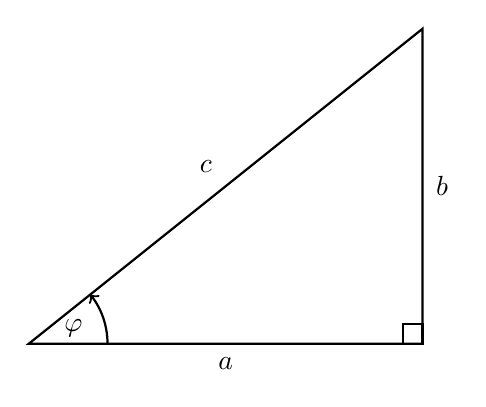
\begin{tikzpicture}[%%
  lineStyle/.style={-,thick},%%
  triangleStyle/.style={-,thick,draw}%%
]
%%
%%
\pgfmathsetmacro{\dx}{0.25}
\pgfmathsetmacro{\dy}{\dx}
\pgfmathsetmacro{\xhigh}{5}
\pgfmathsetmacro{\xlow}{0}
\pgfmathsetmacro{\yhigh}{4}
\pgfmathsetmacro{\ylow}{\xlow}
%%
\coordinate (A) at (\xlow,\ylow);
\coordinate (B) at (\xhigh,\ylow);
\coordinate (C) at (\xhigh,\yhigh);
%%
%% A right-angled triangle.
\path[triangleStyle] (A) -- (B) -- (C) -- cycle;
\draw[lineStyle] (\xhigh-\dx,\ylow) rectangle (\xhigh,\dy);
%% Label the angle.
\path pic["$\varphi$",draw,->,thick,angle radius=1cm] {angle=B--A--C};
%% Label the base.
\node at (\xhigh/2,-\dy) {$a$};
%% Label the height.
\node at (\xhigh+\dx,\yhigh/2) {$b$};
%% Label the hypotenuse.
\node at (\xhigh/2-\dx,\yhigh/2+\dy) {$c$};
\end{tikzpicture}

\end{document}
